%DO NOT MESS AROUND WITH THE CODE ON THIS PAGE UNLESS YOU %REALLY KNOW WHAT YOU ARE DOING
\chapter*{Experimental Research}
\addcontentsline{toc}{chapter}{Experimental Research}


\section{ Surface Backscattering } \label{ Surface Backscattering } 
\noindent  We can see the effect of varying wind speed and frequency on surface reverberation from figure 3.1 and figure 3.2. It can be depicted that as the wind speed increases, roughness of the surface increases and hence higher is the backscattering. Surface reverberation increases non-linearly with increase in grazing angle. At a particular wind speed if the frequency is varied between 50 kHz to 400 kHz, the surface reverberation remains almost constant. For lower wind speeds surface reverberation increase is not significantly observed. At wind speed of 40 knots, we can see that with increase in frequency there is slight nonlinear increase in the surface backscattering coefficient.

\begin{figure}[H]
\centering
{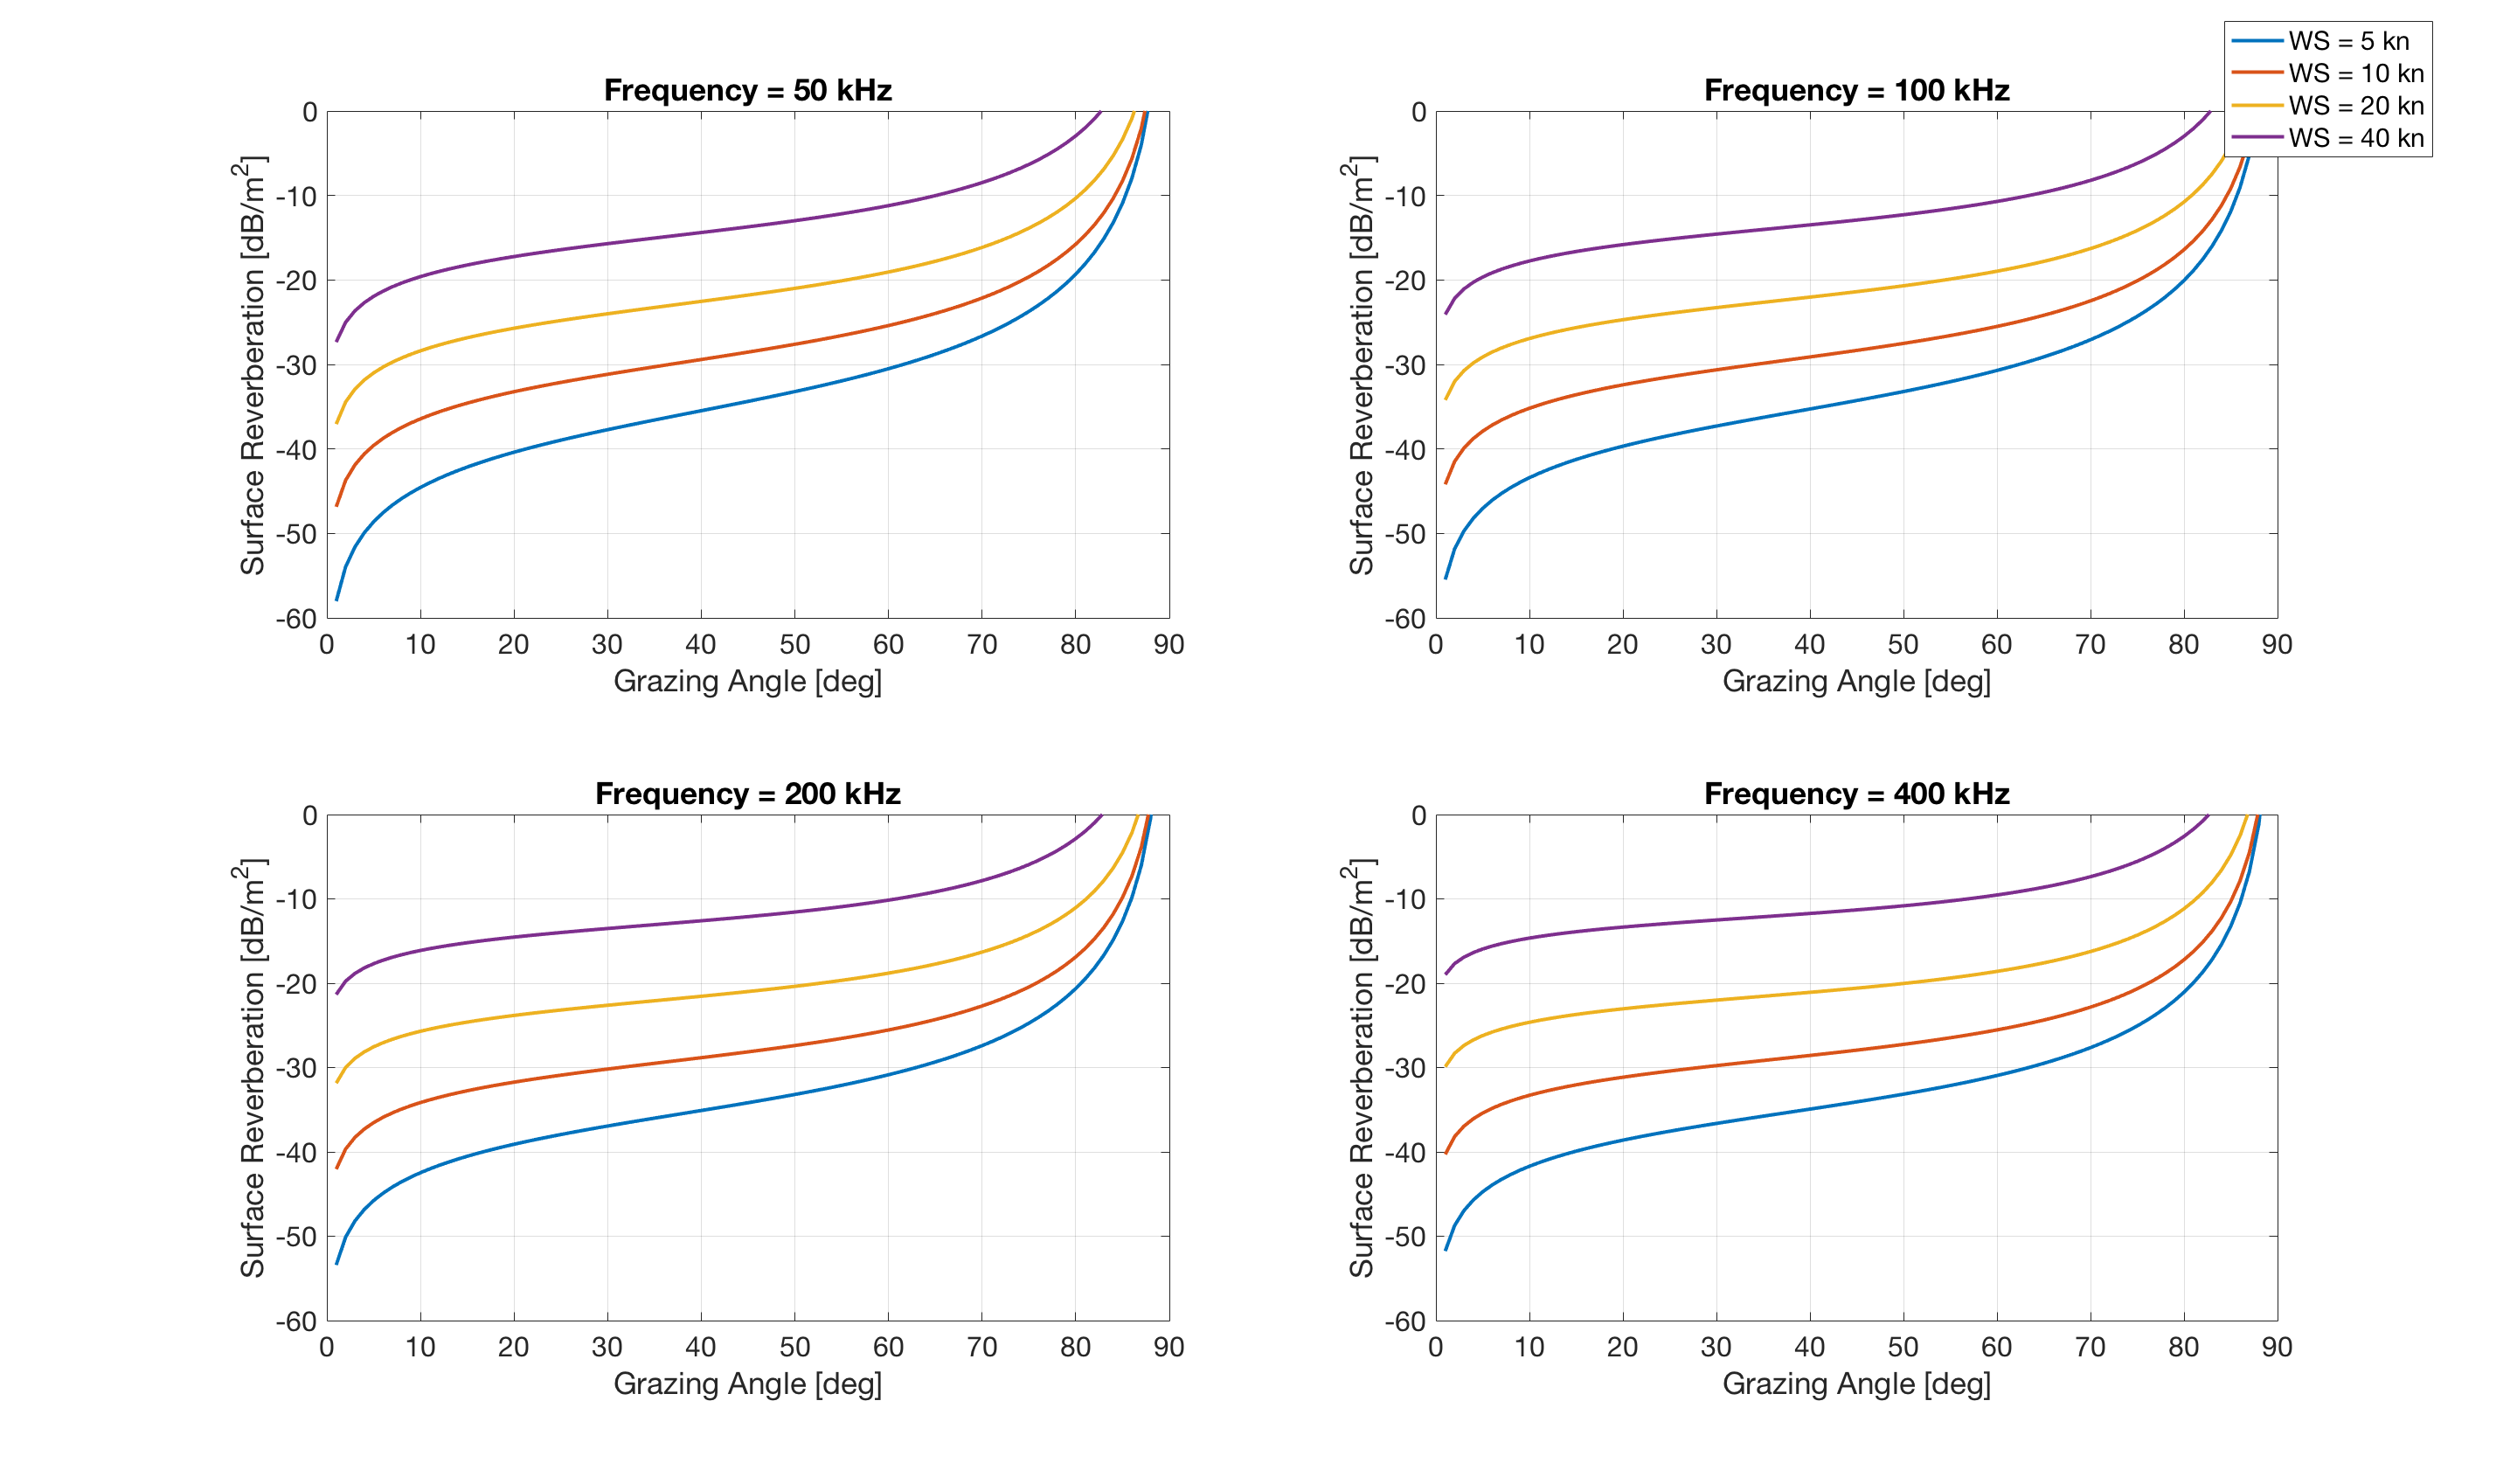
\includegraphics[scale=0.18]{usp3_1.png}}
\caption{Surface reverberation versus grazing angle for frequency dependency}
\end{figure}

\begin{figure}[H]
\centering
{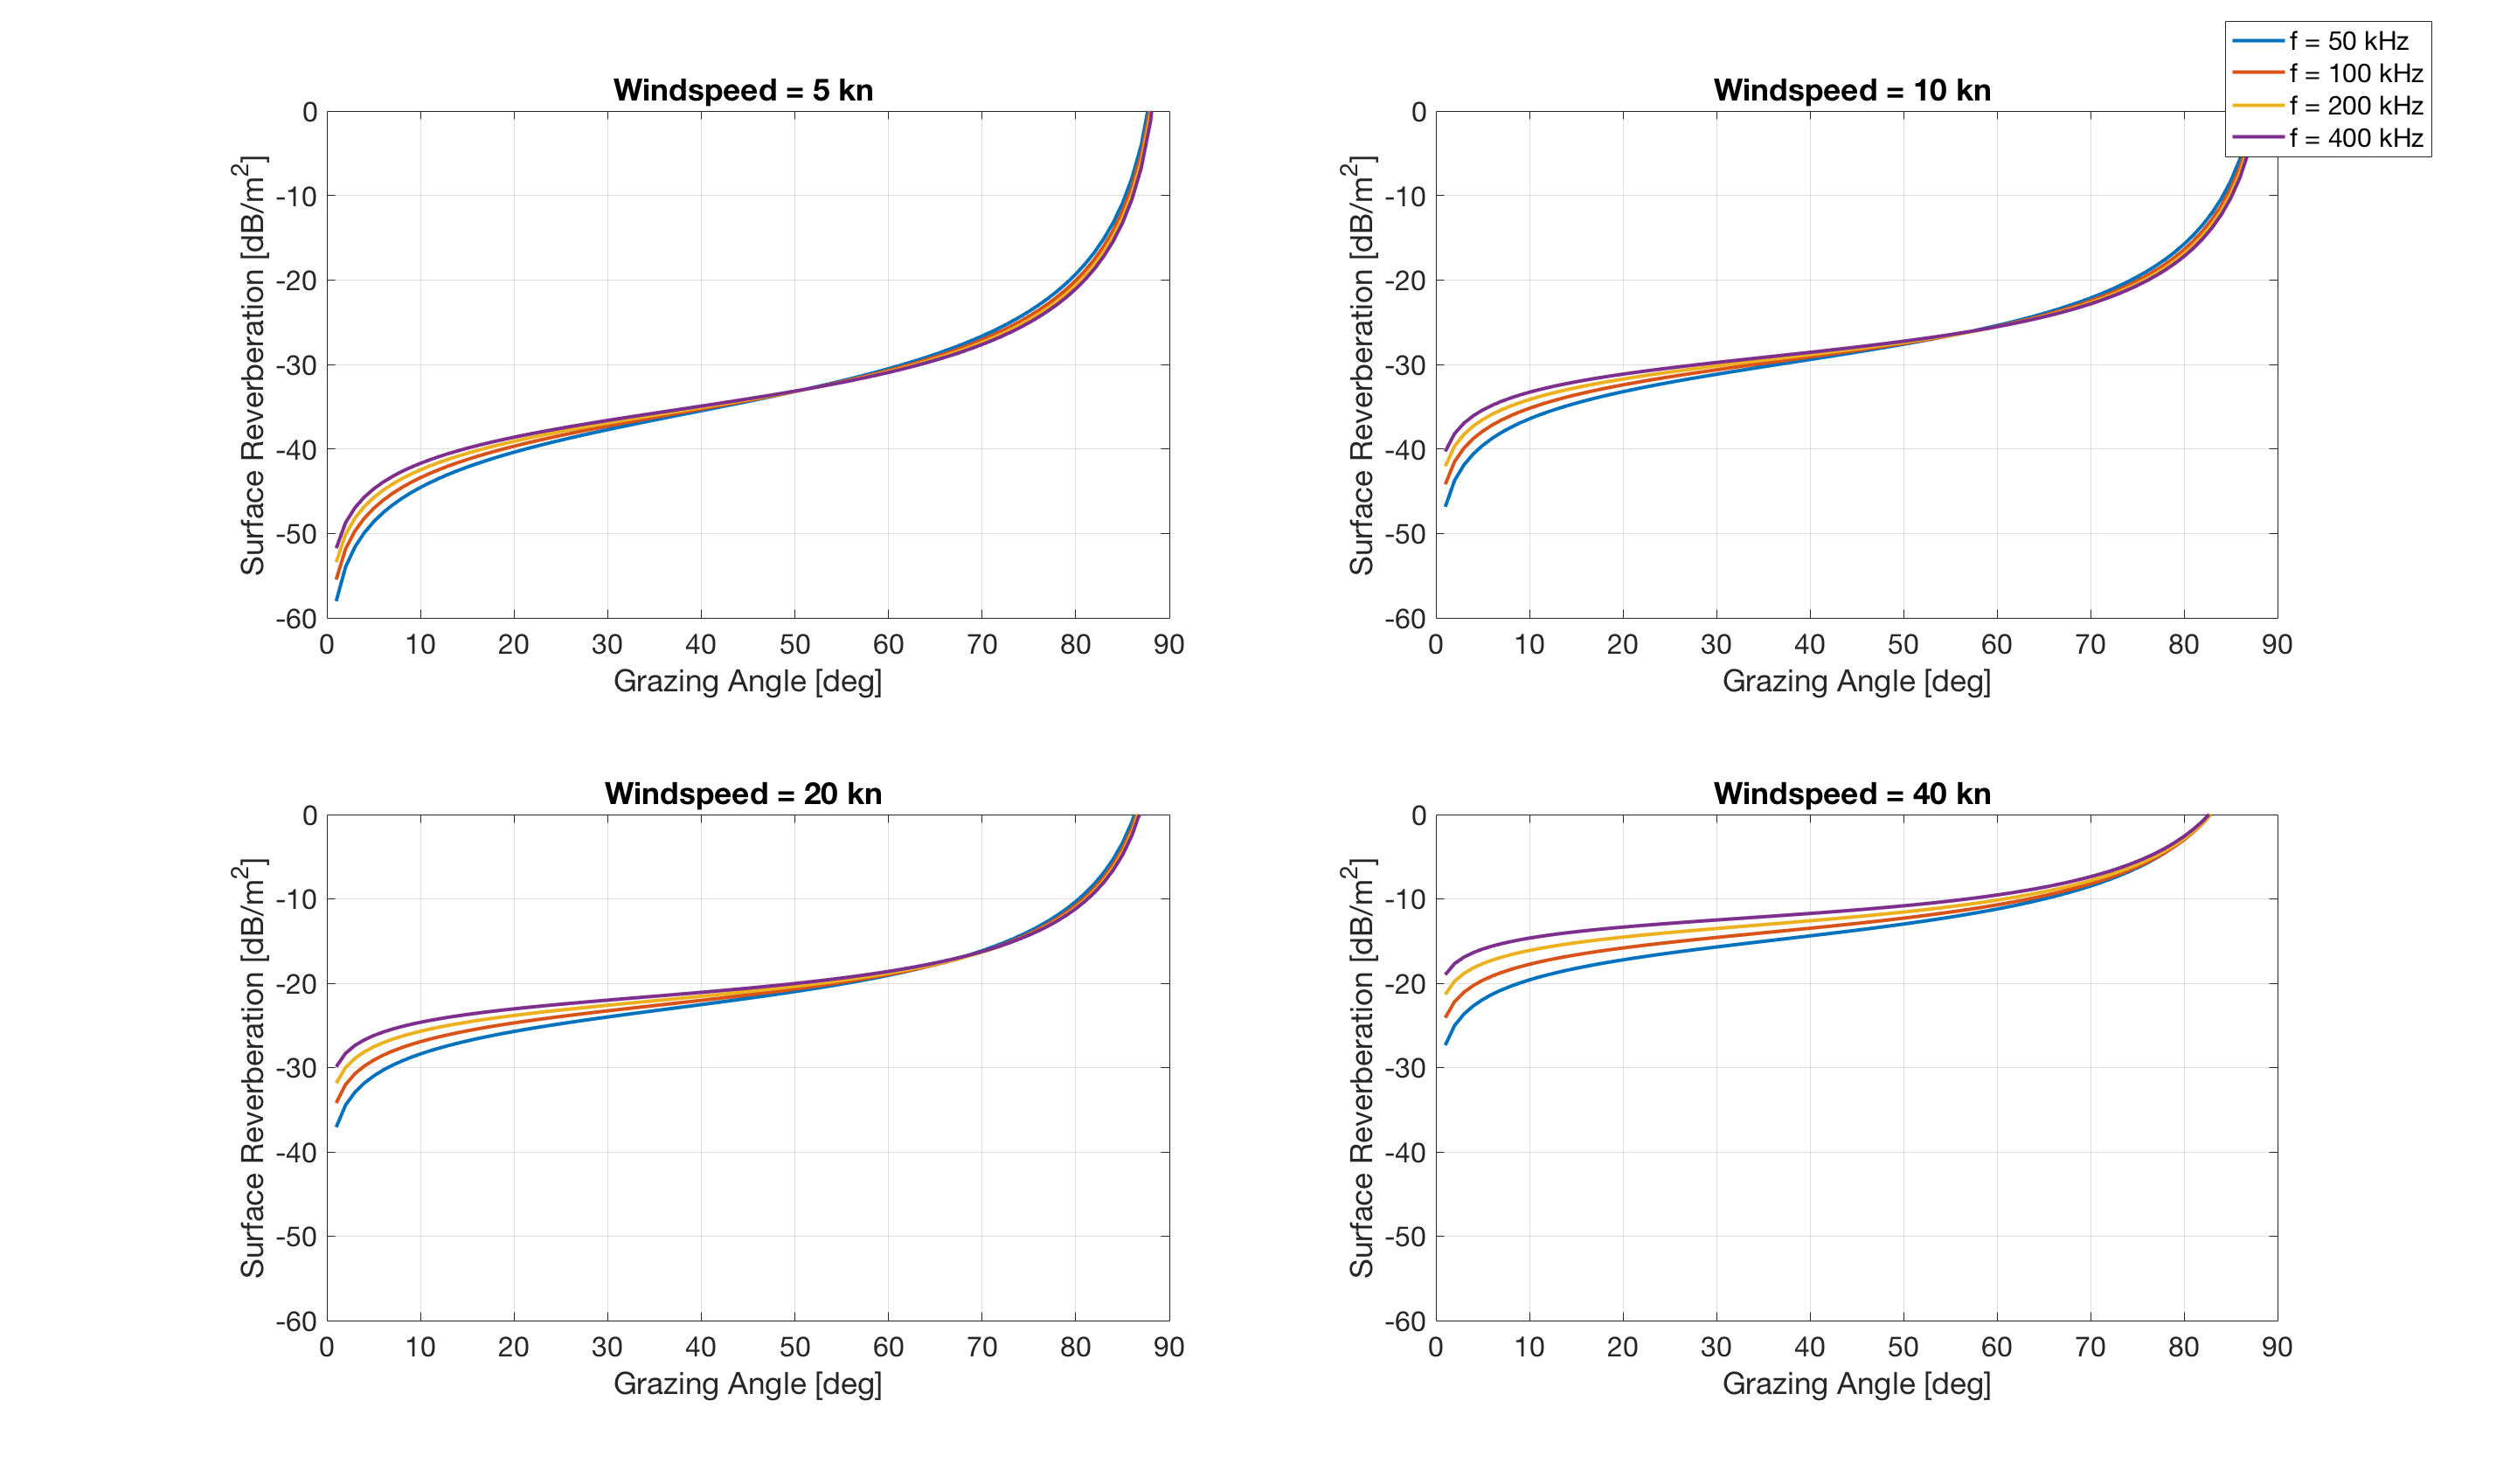
\includegraphics[scale=0.18]{usp3_2.png}}
\caption{Surface reverberation versus grazing angle for wind speed dependency}
\end{figure}

\newpage

\section{ Bottom Backscattering } \label{ Bottom Backscattering } 
\noindent We can see the effect of varying bottom type and frequency on reverberation from figure 3.3 and figure 3.4. Reverberation increases non-linearly with grazing angle for different bottom types. At any frequency (here 50 kHz to 400 kHz), reverberation is lowest for mud (\textit{bt} = 1). For grazing angles between $0^{\circ}$ to $60^{\circ}$, maximum reverberation is observed for rock (\textit{bt} = 4). As the frequency increases, reverberation for the sand (\textit{bt} = 2) increases more than other bottom types for grazing angles greater than $60^{\circ}$. For bottom type mud (\textit{bt} = 1), as the frequency is increased from 50 kHz to 400 kHz, the reverberation level increases from -40 dB to -30 dB. As the bottom type becomes harder from mud to rock (\textit{bt} increases from 1 to 4), we can see lesser variations in reverberation with increasing frequency. For bottom type rock (\textit{bt} = 4), reverberation becomes independent of frequency level. 

\begin{figure}[H]
\centering
{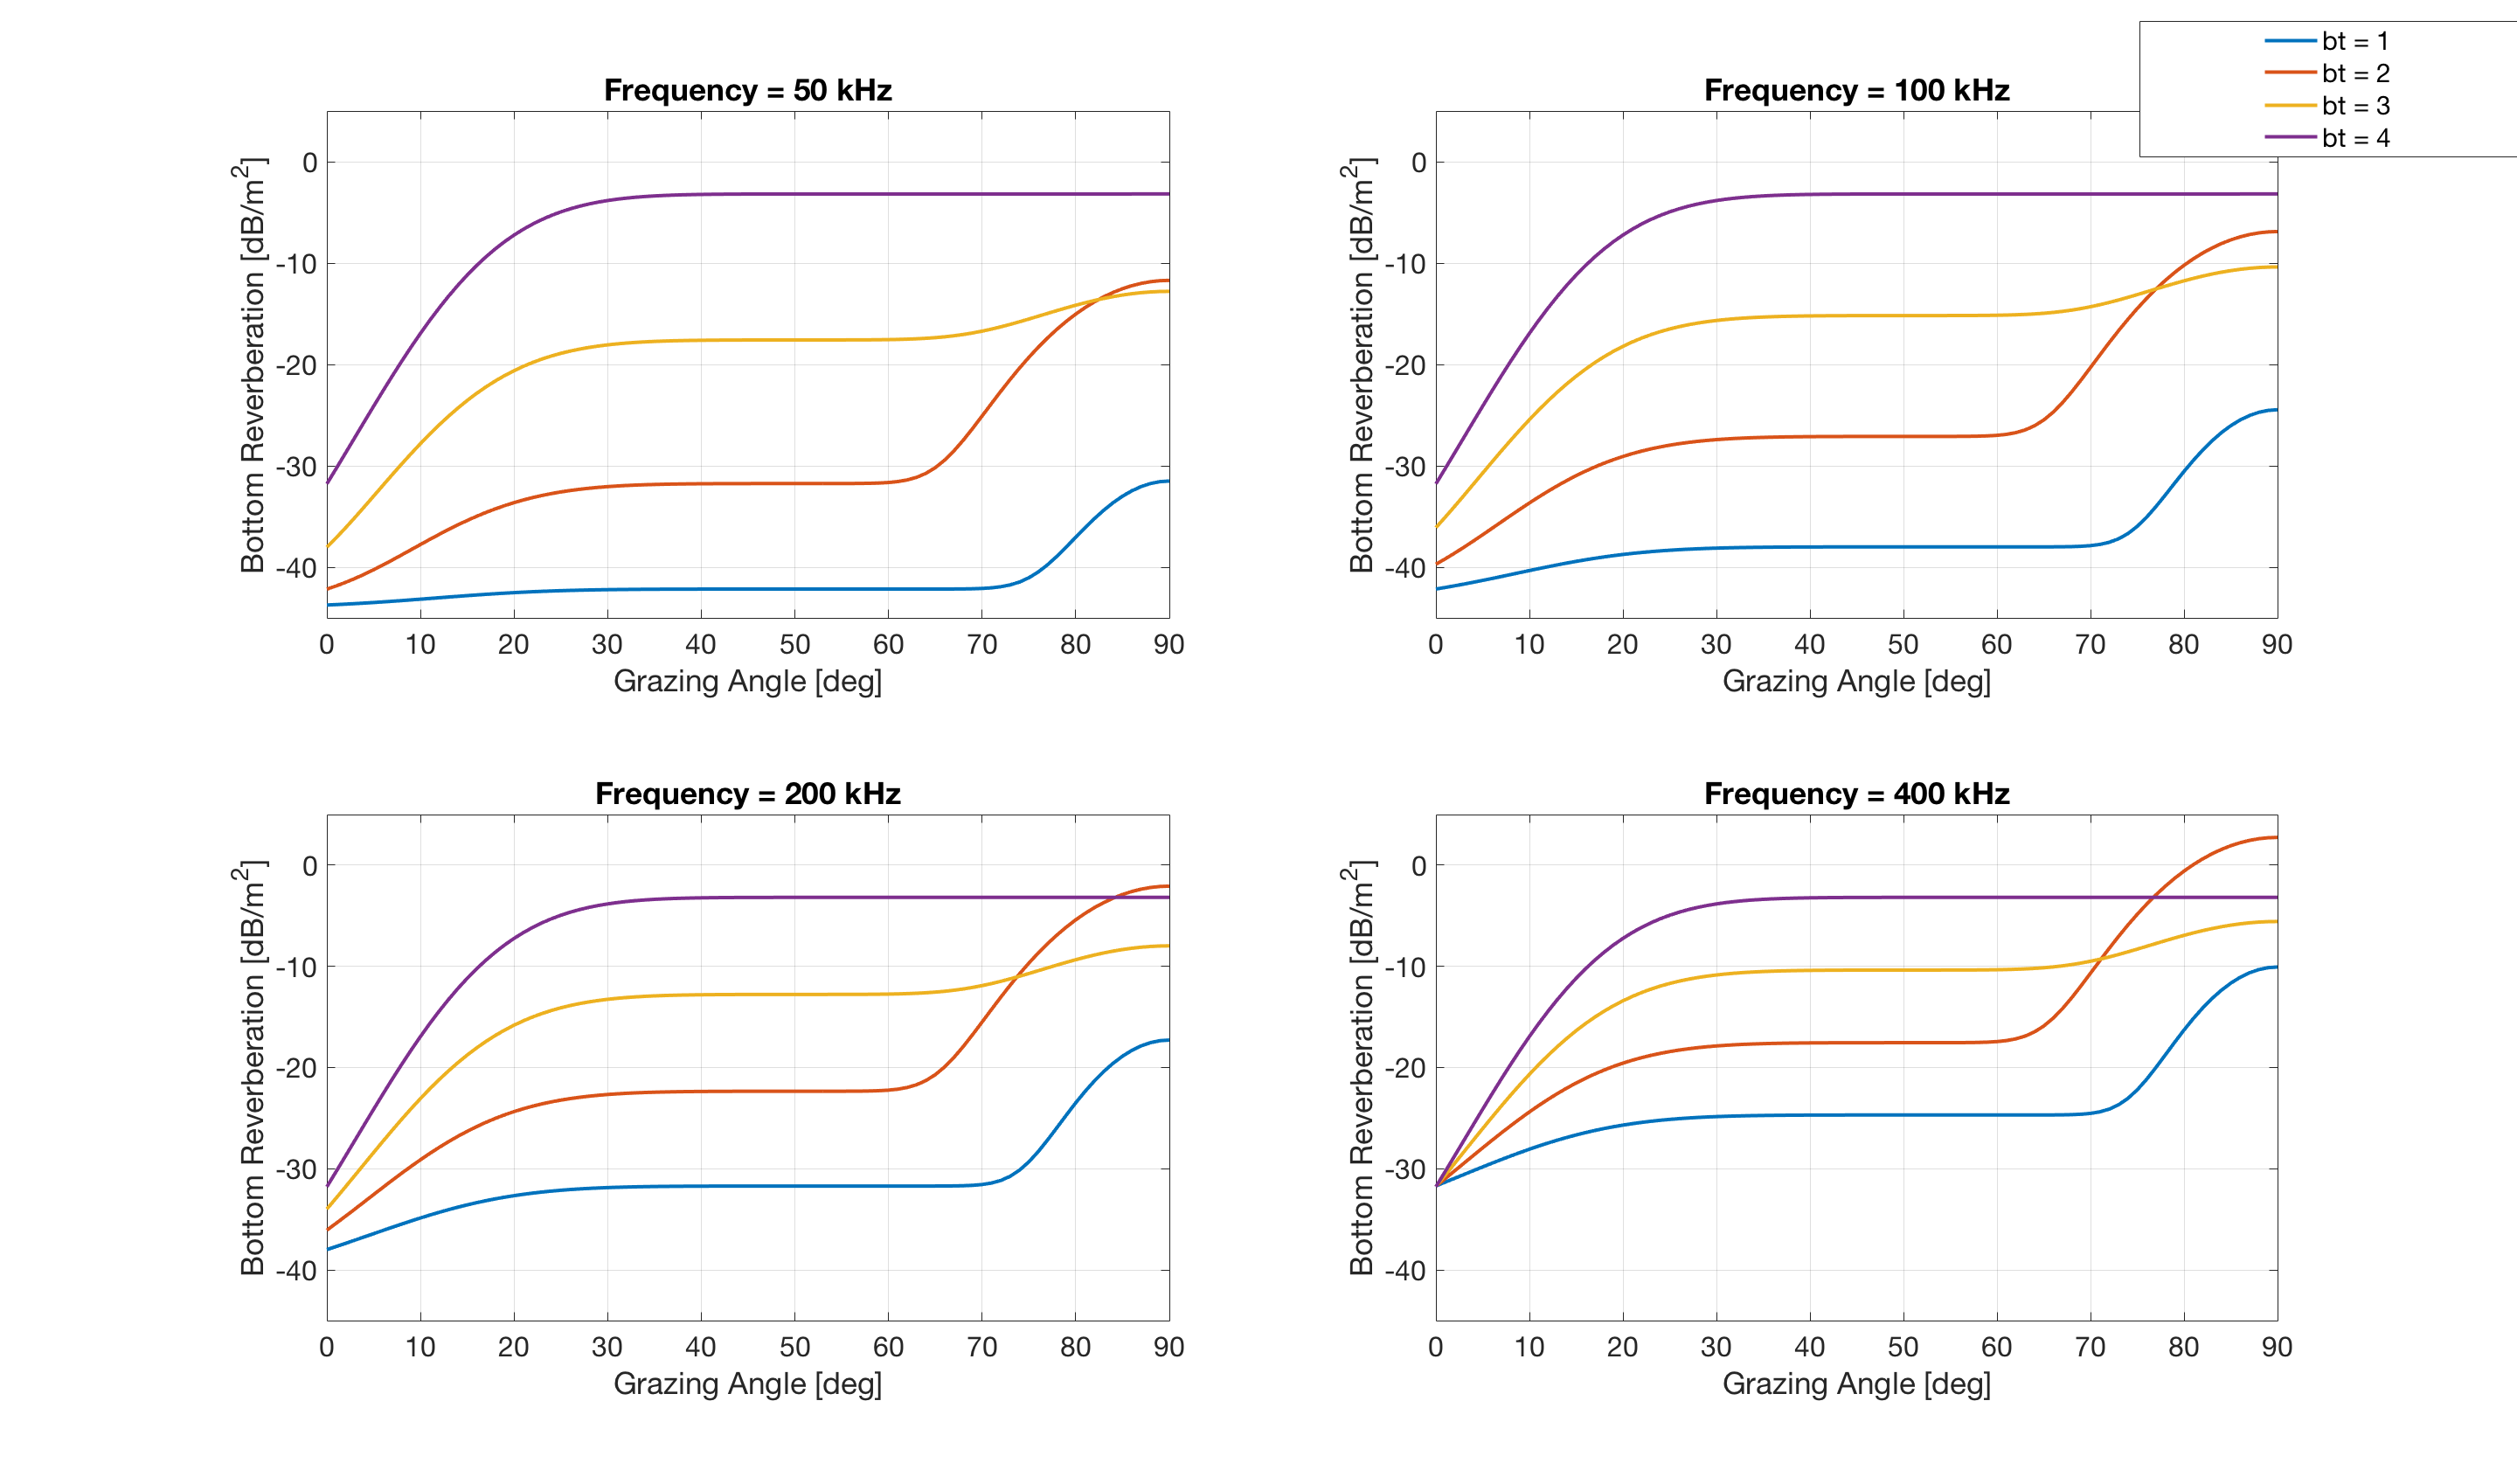
\includegraphics[scale=0.18]{usp3_3.png}}
\caption{Bottom reverberation versus grazing angle for frequency dependency}
\end{figure}

\begin{figure}[H]
\centering
{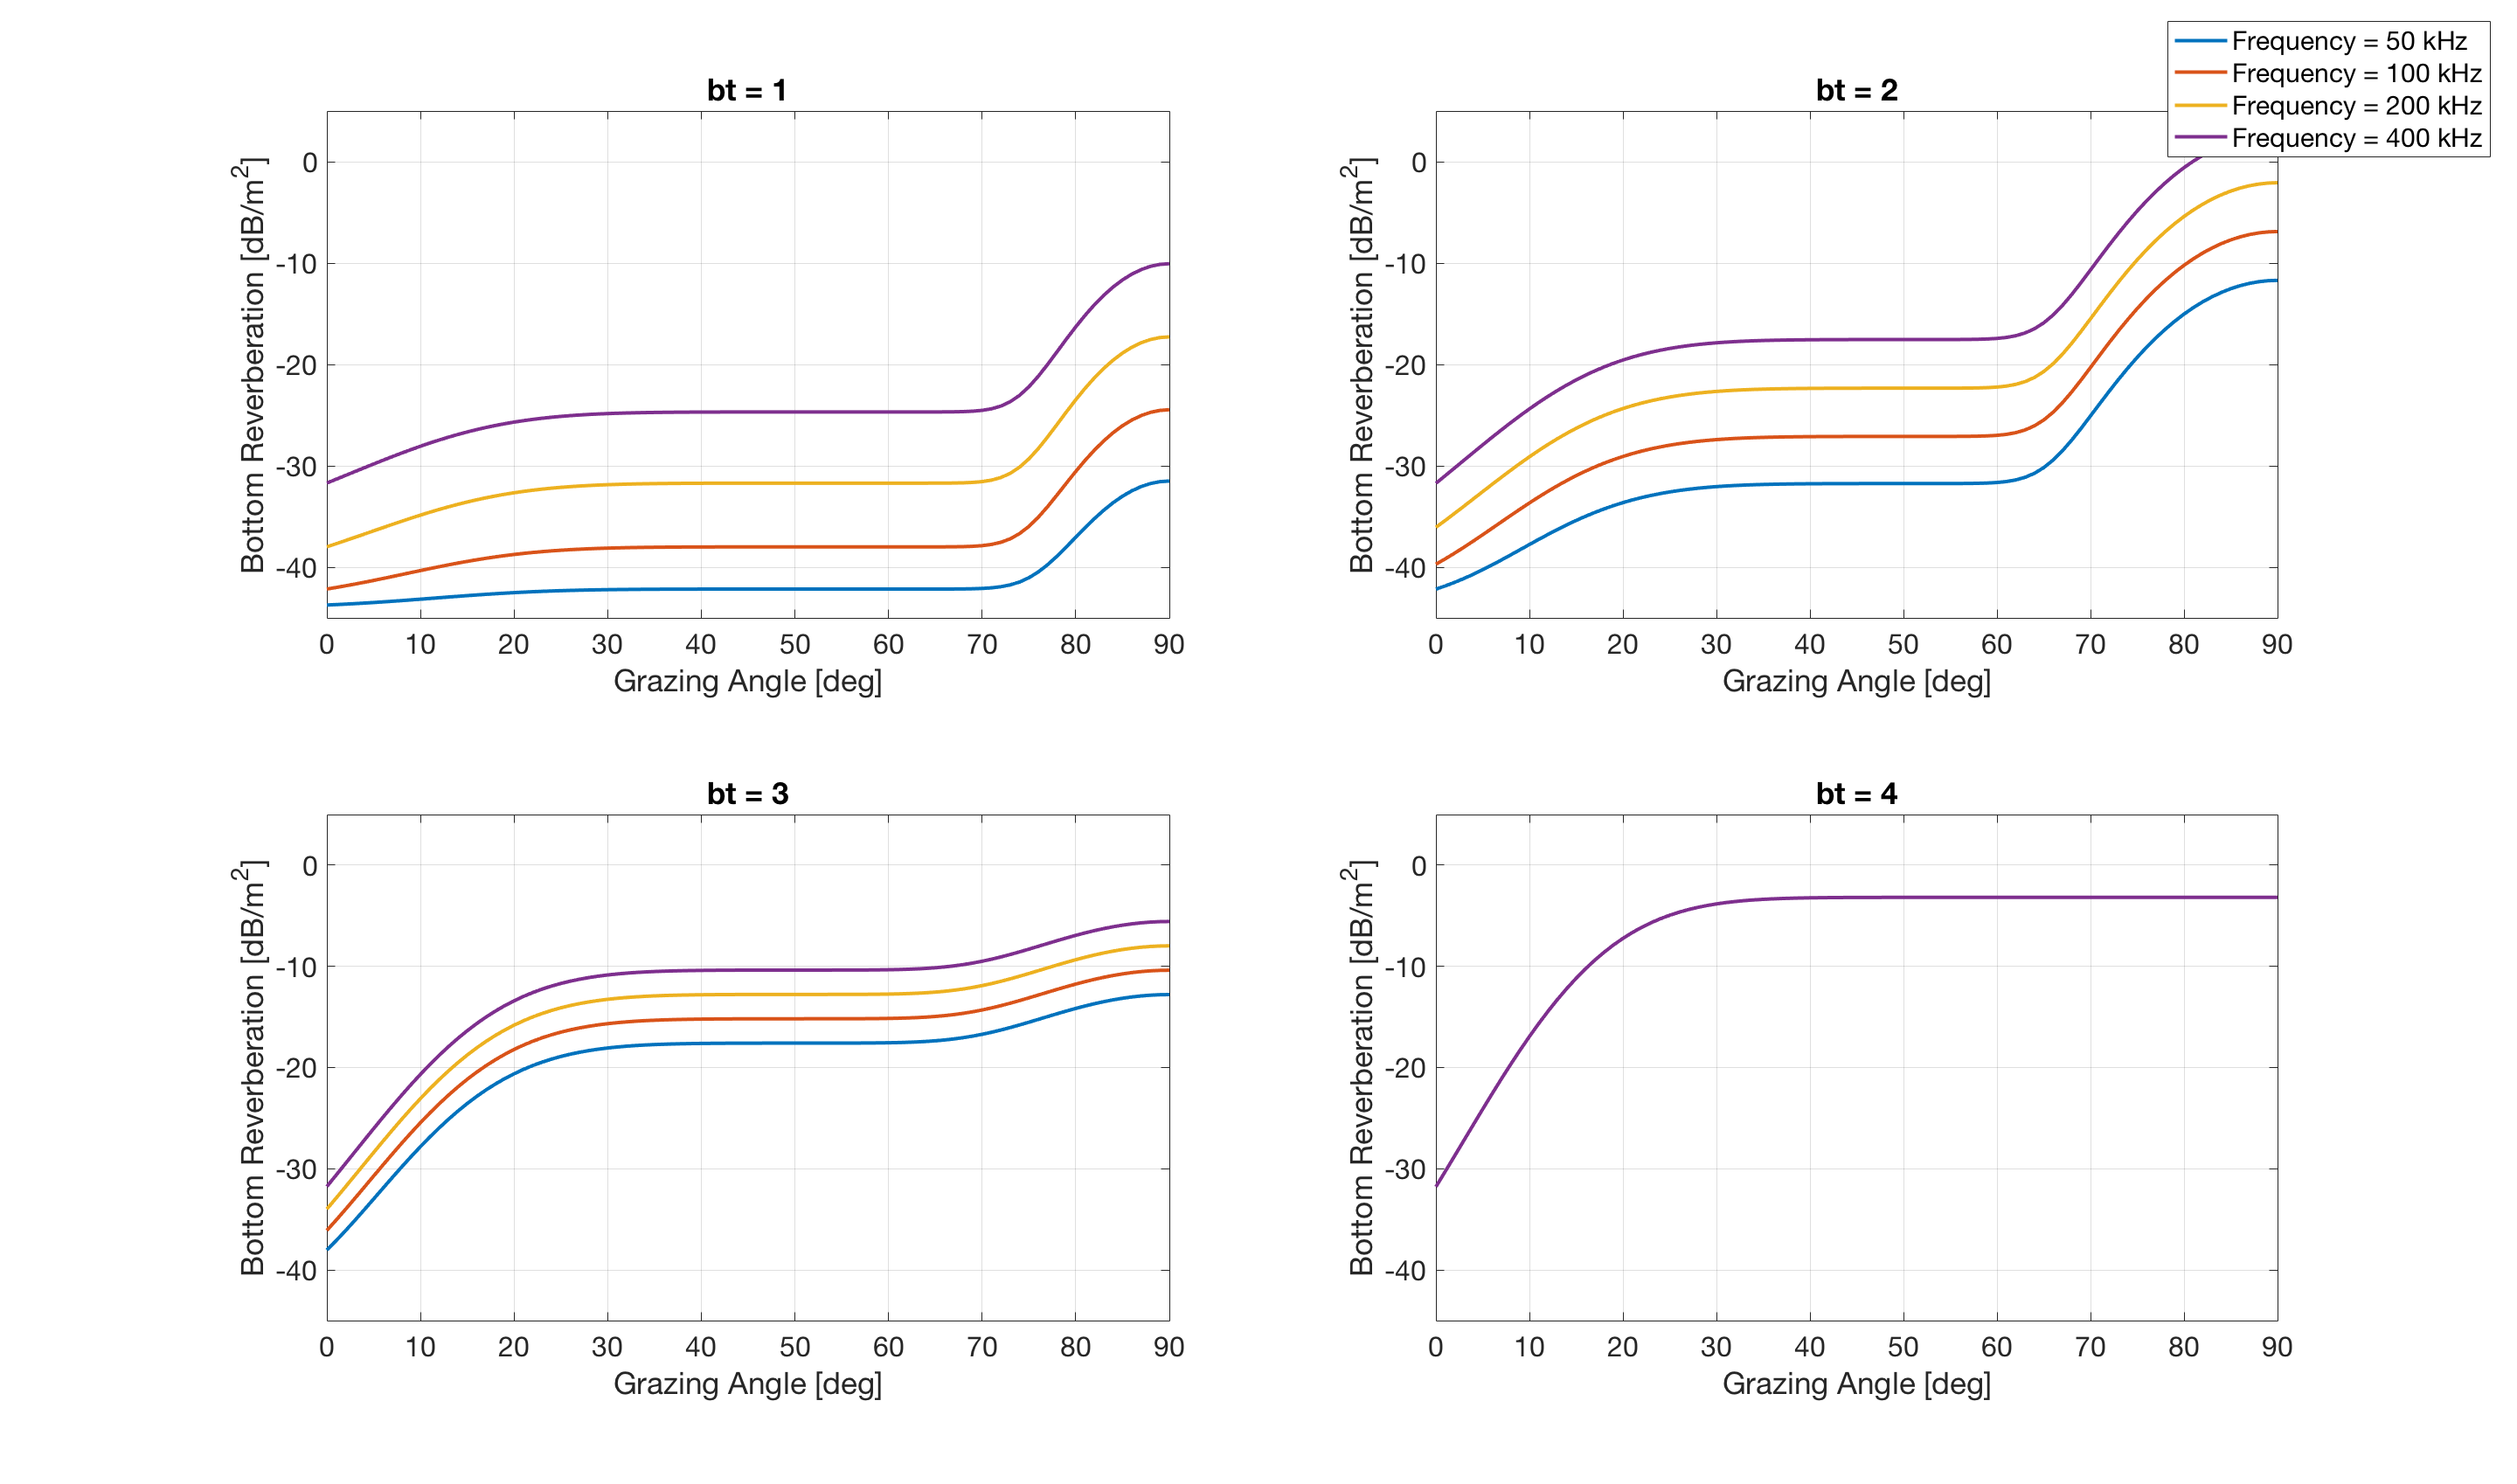
\includegraphics[scale=0.18]{usp3_4.png}}
\caption{Bottom reverberation versus grazing angle for bottom-type dependency}
\end{figure}

\newpage

\section{ Volume Backscattering } \label{ Volume Backscattering } 
\noindent From figure 3.5, we can say that when the particle density is higher, then the volume reverberation is higher. Particle density can be influenced by biological organisms and turbidity underwater. Volume reverberation increases non linearly with the increase in frequency for particular particle density value. 

\begin{figure}[H]
\centering
{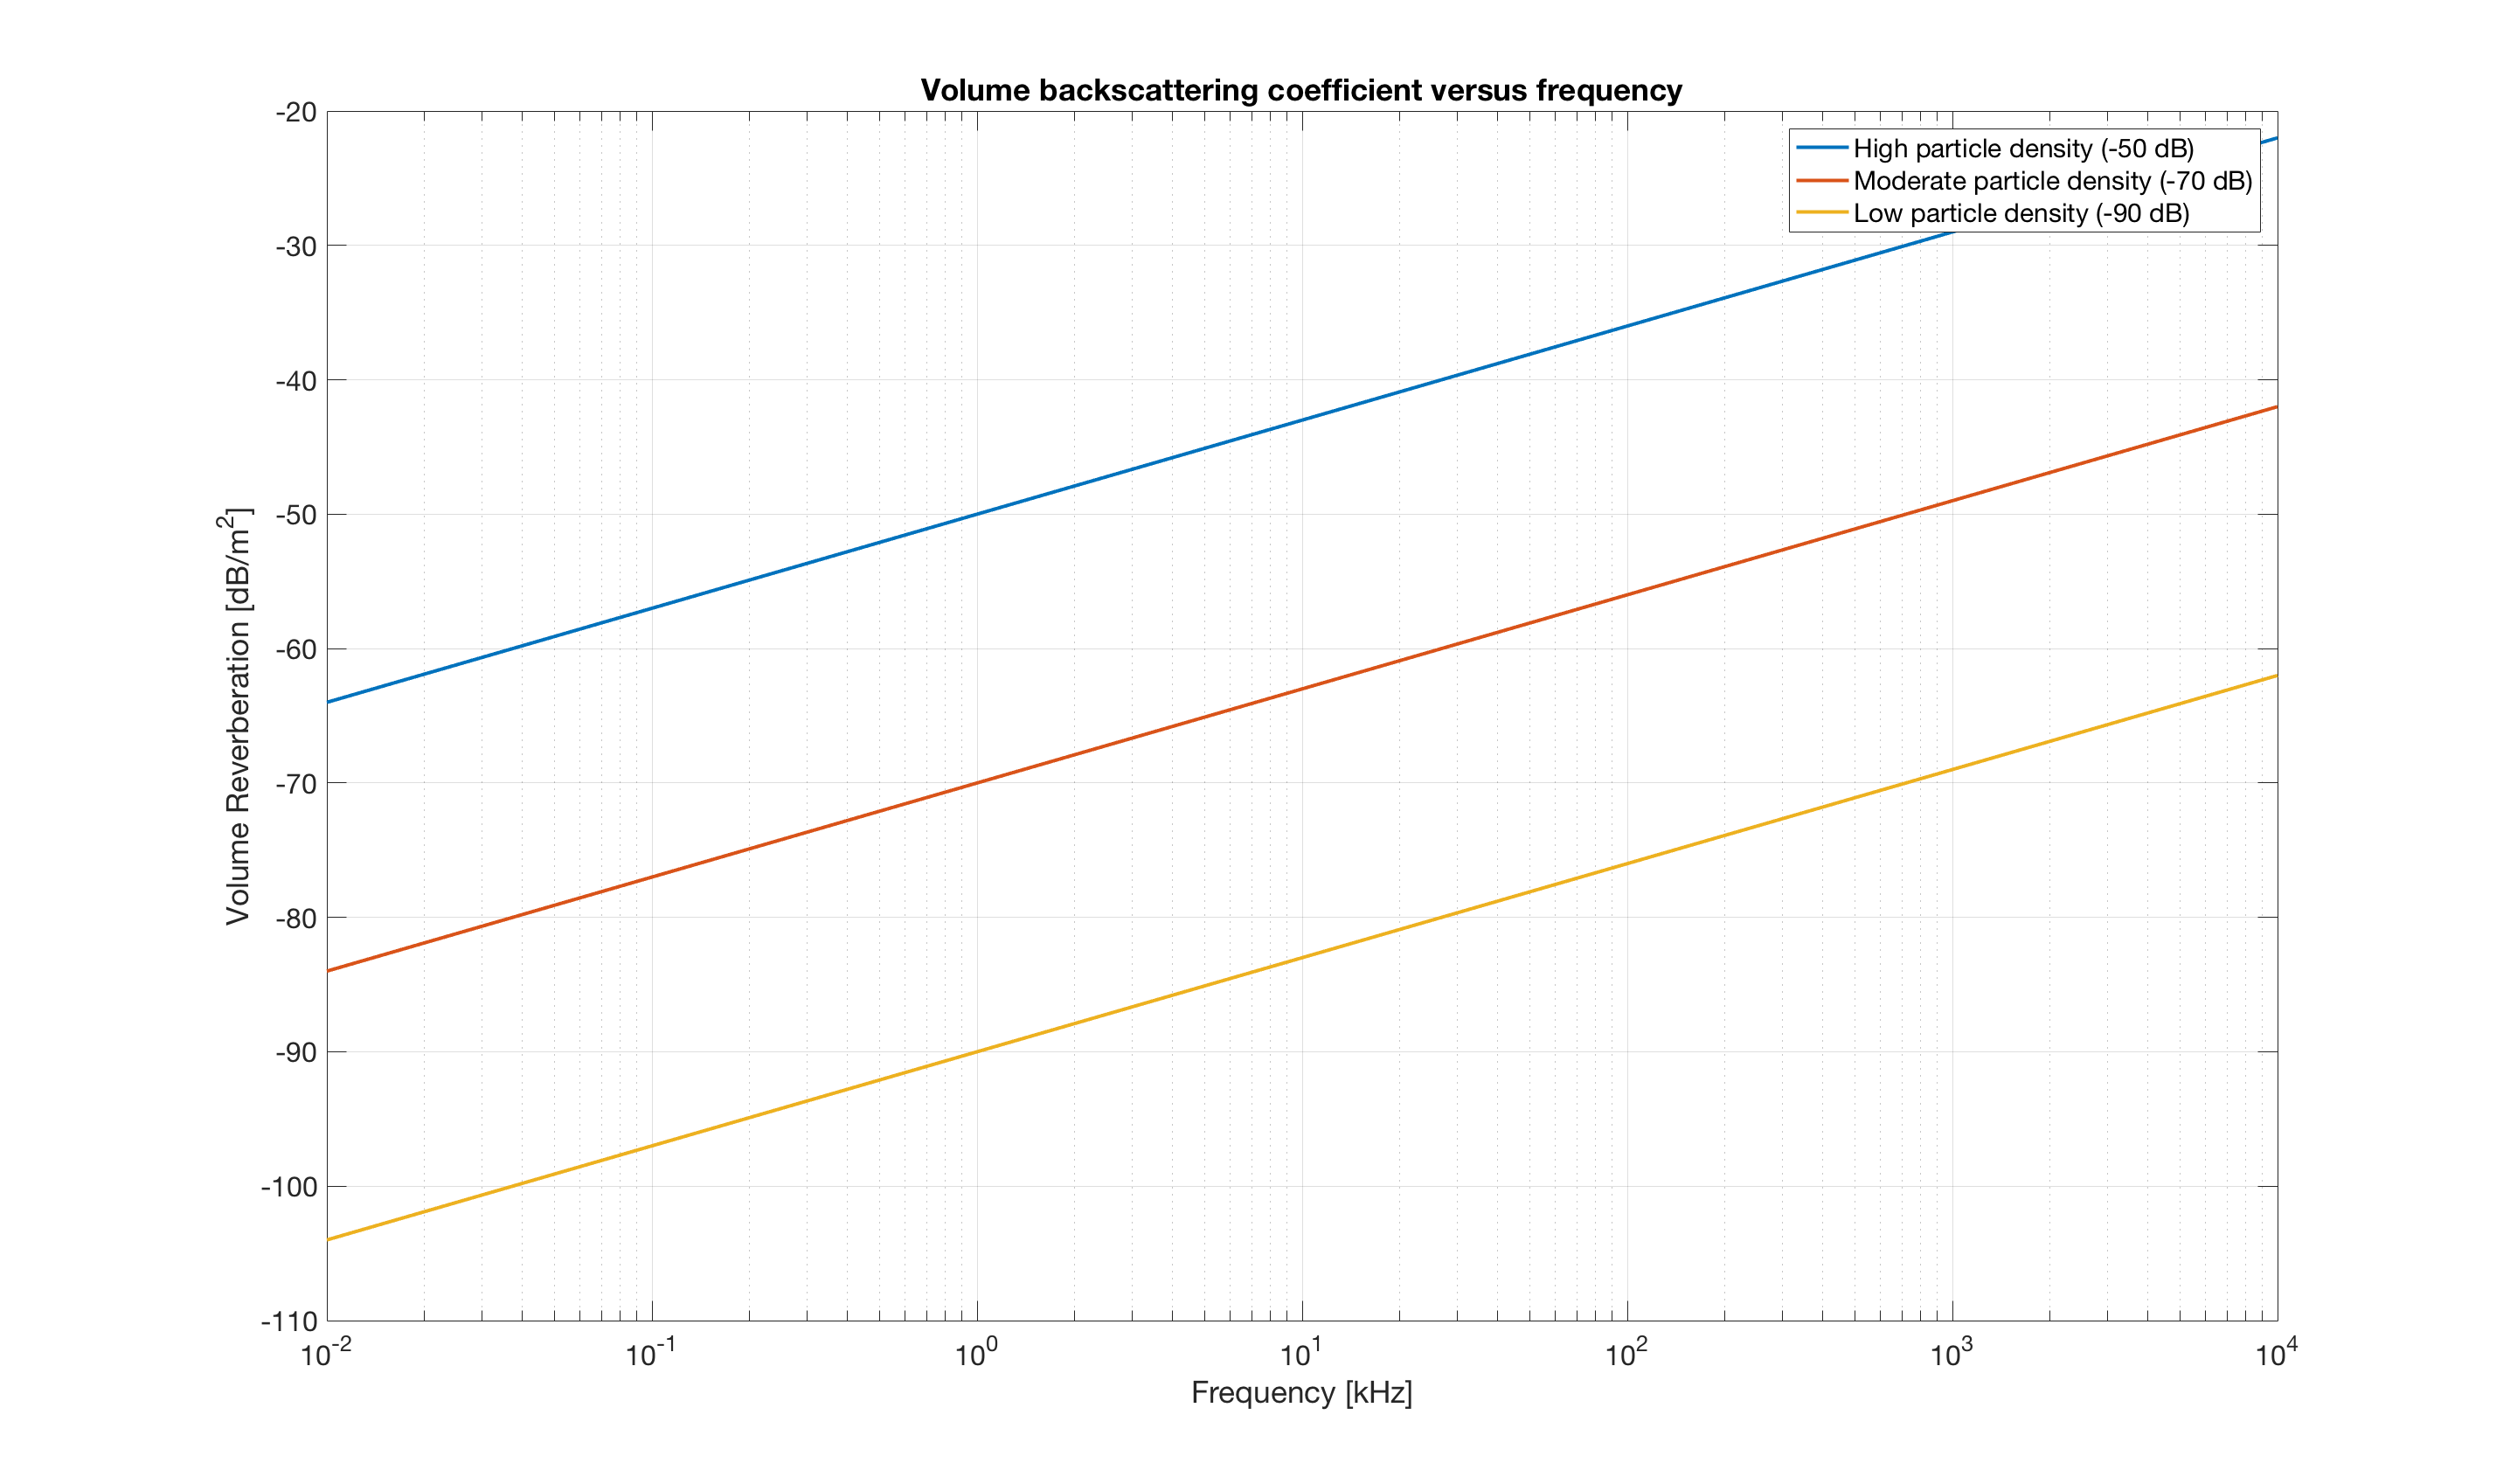
\includegraphics[scale=0.18]{usp3_5.png}}
\caption{Volume reverberation versus frequency for various particle densities}
\end{figure}



